\documentclass[11pt]{amsart}

\usepackage{amsmath,amsthm}
\usepackage{amssymb}
\usepackage{graphicx}
\usepackage{enumerate}
\usepackage{fullpage}
\usepackage{tikz-cd}
% \usepackage{euscript}
% \makeatletter
% \nopagenumbers
\usepackage{verbatim}
\usepackage{color}
\usepackage{hyperref}

\usepackage{fullpage,tikz,float}
%\usepackage{times} %, mathtime}

\textheight=600pt %574pt
\textwidth=480pt %432pt
\oddsidemargin=15pt %18.88pt
\evensidemargin=18.88pt
\topmargin=10pt %14.21pt

\parskip=1pt %2pt

% define theorem environments
\newtheorem{theorem}{Theorem}    %[section]
%\def\thetheorem{\unskip}
\newtheorem{proposition}[theorem]{Proposition}
%\def\theproposition{\unskip}
\newtheorem{conjecture}[theorem]{Conjecture}
\def\theconjecture{\unskip}
\newtheorem{corollary}[theorem]{Corollary}
\newtheorem{lemma}[theorem]{Lemma}
\newtheorem{sublemma}[theorem]{Sublemma}
\newtheorem{fact}[theorem]{Fact}
\newtheorem{observation}[theorem]{Observation}
%\def\thelemma{\unskip}
\theoremstyle{definition}
\newtheorem{definition}{Definition}
%\def\thedefinition{\unskip}
\newtheorem{notation}[definition]{Notation}
\newtheorem{remark}[definition]{Remark}
% \def\theremark{\unskip}
\newtheorem{question}[definition]{Question}
\newtheorem{questions}[definition]{Questions}
%\def\thequestion{\unskip}
\newtheorem{example}[definition]{Example}
%\def\theexample{\unskip}
\newtheorem{problem}[definition]{Problem}
\newtheorem{exercise}[definition]{Exercise}

\numberwithin{theorem}{section}
\numberwithin{definition}{section}
\numberwithin{equation}{section}

\def\reals{{\mathbb R}}
\def\torus{{\mathbb T}}
\def\integers{{\mathbb Z}}
\def\rationals{{\mathbb Q}}
\def\naturals{{\mathbb N}}
\def\complex{{\mathbb C}\/}
\def\distance{\operatorname{distance}\,}
\def\support{\operatorname{support}\,}
\def\dist{\operatorname{dist}\,}
\def\Span{\operatorname{span}\,}
\def\degree{\operatorname{degree}\,}
\def\kernel{\operatorname{kernel}\,}
\def\dim{\operatorname{dim}\,}
\def\codim{\operatorname{codim}}
\def\trace{\operatorname{trace\,}}
\def\dimension{\operatorname{dimension}\,}
\def\codimension{\operatorname{codimension}\,}
\def\nullspace{\scriptk}
\def\kernel{\operatorname{Ker}}
\def\p{\partial}
\def\Re{\operatorname{Re\,} }
\def\Im{\operatorname{Im\,} }
\def\ov{\overline}
\def\eps{\varepsilon}
\def\lt{L^2}
\def\curl{\operatorname{curl}}
\def\divergence{\operatorname{div}}
\newcommand{\norm}[1]{ \|  #1 \|}
\def\expect{\mathbb E}
\def\bull{$\bullet$\ }
\def\det{\operatorname{det}}
\def\Det{\operatorname{Det}}
\def\rank{\mathbf r}
\def\diameter{\operatorname{diameter}}

\def\t2{\tfrac12}

\newcommand{\abr}[1]{ \langle  #1 \rangle}

\def\newbull{\medskip\noindent $\bullet$\ }
\def\field{{\mathbb F}}
\def\cc{C_c}



% \renewcommand\forall{\ \forall\,}

% \newcommand{\Norm}[1]{ \left\|  #1 \right\| }
\newcommand{\Norm}[1]{ \Big\|  #1 \Big\| }
\newcommand{\set}[1]{ \left\{ #1 \right\} }
%\newcommand{\ifof}{\Leftrightarrow}
\def\one{{\mathbf 1}}
\newcommand{\modulo}[2]{[#1]_{#2}}

\def\bd{\operatorname{bd}\,}
\def\cl{\text{cl}}
\def\nobull{\noindent$\bullet$\ }

\def\scriptf{{\mathcal F}}
\def\scriptq{{\mathcal Q}}
\def\scriptg{{\mathcal G}}
\def\scriptm{{\mathcal M}}
\def\scriptb{{\mathcal B}}
\def\scriptc{{\mathcal C}}
\def\scriptt{{\mathcal T}}
\def\scripti{{\mathcal I}}
\def\scripte{{\mathcal E}}
\def\scriptv{{\mathcal V}}
\def\scriptw{{\mathcal W}}
\def\scriptu{{\mathcal U}}
\def\scriptS{{\mathcal S}}
\def\scripta{{\mathcal A}}
\def\scriptr{{\mathcal R}}
\def\scripto{{\mathcal O}}
\def\scripth{{\mathcal H}}
\def\scriptd{{\mathcal D}}
\def\scriptl{{\mathcal L}}
\def\scriptn{{\mathcal N}}
\def\scriptp{{\mathcal P}}
\def\scriptk{{\mathcal K}}
\def\scriptP{{\mathcal P}}
\def\scriptj{{\mathcal J}}
\def\scriptz{{\mathcal Z}}
\def\scripts{{\mathcal S}}
\def\scriptx{{\mathcal X}}
\def\scripty{{\mathcal Y}}
\def\frakv{{\mathfrak V}}
\def\frakG{{\mathfrak G}}
\def\aff{\operatorname{Aff}}
\def\frakB{{\mathfrak B}}
\def\frakC{{\mathfrak C}}

\def\symdif{\,\Delta\,}
\def\mustar{\mu^*}
\def\muplus{\mu^+}

\def\soln{\noindent {\bf Solution.}\ }


%\pagestyle{empty}
%\setlength{\parindent}{0pt}

\begin{document}

\begin{center}{\bf Math 215A --- Homework 12--- UCB, Spring 2017 --- William Guss} \\
Partners: Alekos, Chris \\
Selected Problems: 2
\end{center}


\medskip \noindent {\bf (13.2)}\ \emph{(Alexander's Horned Ball)} Let $f: D^3 \to \mathbb{R}^3$ be the embedding of Alexander's horned ball, whose compliment $C$ is not simply-connected. Consider a meridian circle $\mu \subset C$, i.e., an embedded circle that goes once around the thick red part at the bottom of largest 'loop' in $f$. Draw a compact oriented surface in $C$ whose boundary is $\mu$ and conclude that $\mu$ represents the trivial element in $H_1(C)$. Explain why $\mu$ cannot be null-homotopic. 

\medskip \noindent \emph{Solution.} First, we will show that $\pi_1(C) \neq 0$ and that $\mu$ cannot be null-homotopic. Recall the following proposition.
\begin{proposition}
  	If $X$ is a simply connected if and only if it is path connected and $\pi_1(X, x_0)$ is trivial for all $x_0 \in X.$
  \end{proposition}  
  \begin{proof}
  	Suppose that $X$ is simply connected. Now any loop $f: I \to X$ with $f(0)= f(1) = x_0$  is equivalent to a continuous map $f: S^1 \to X$ by quotienting the endpoints of $I$. By definition $X$ is path connected and any continuous map $f: S^1 \to X$ can be contracted to a point in the following sense: there exists a continuous map $F: D^2 \to X$ such that $F$ restricted to $S^1$ is $f$. Chose any $\theta_0 \in S^1$ and let $f(\theta_0) = x_0$ be a basepoint of $X.$ Then $F$ parameterized by polar coordinates is a homtopy of $f$ to the constant loop $c_{x_0}$. Therefore $\pi_1(X, x_0) = [c_{x_0}]_\simeq \cong \{0\}$, and since $X$ is path connected, $\pi_1(X, x_0) \cong \pi_1(X, y)$ for all $y \in X$. 

  	In the converse direction, if $\pi_1(X, x_0) = 0$ for every $x_0$ and $X$ is path connected then any loop $f \in [c_{x_0}]_\simeq$ is equivalently continuous map $f: S^1 \to X$. The homotopy of $h: I^2 \to X$ of $f$ to $c_{x_0}$ is equivalently a continuous map $F: D^2 \to X$ via the homeomorphic reparameterizion $D^2 \cong I^2$, and so every continuous map $f: S^1 \to X$ extends to a continuous map $F: D^2 \to X$, and choice of $x_0$ is arbitrary so all such $f$ are expressed. Therefore $X$ is simply connected.
  \end{proof}

  By the proposition, since $C$ is not simply connected\footnote{See Hatcher}, the $\pi_1(C) \neq \{0\}$. In particular $\mu$ cannot be homotoped to the zero map. To see this, 
  recall Hatcher's construction with finite stages of $C$, denoted $Y_n= \mathbb{R}^3 \setminus X_n$ with $X_n$ the $n$th stage of the construction of the horned  ball. Using $\mu \in \pi_1(Y_0) = \mathbb{Z}$ and using Van Kampen's theorem it can be shwon that $\pi_1(Y_{n})$ injects $\pi_1(Y_{n+1});$ this argument is more rigorously established by Hatcher. Furthermore each loop in $C$ has a compact image and is contained in some $Y_{n}$ and futhermore the homotopies of these loops must becontained within $Y_n$. Thus $\pi_1(C)$ is isomorphic to the union $\bigcup_{n =0}^\infty\pi_1(Y_n)$. Because $[\mu]_{\simeq} \in\pi_1(Y_0)$ is not contractible ($Y_0$ is the compliment of the solid torus), $[\mu]_{\simeq} \in \pi_1(C)$ is not contractible.  Geometrically speaking (informally) , pulling $\mu$ along one of the two initial horns would then require that it be unraveled along each of $2^n$ tips at each $X_n$ and the limit over the stages of the homotopies of $\mu$ to the constant map at each stage doesn't appear continuous.
\newpage
  Now we will draw a compact oriented surface with whose boundary is $\mu.$  The classification of surfaces of boundary gives that any orientable surface with boundary is the connected sum of spheres or tori with a number of open disks removed. Therefore we will focus on how the connected sum of tori or spheres with $1$ open disk removed can embed into $C$ such that the boundary of the embedding is $\mu$. First consider $S^1 \setminus (D^1)^o$ as follows: at stage $c_1$ we will wrap the right half of the partial torus with a hemisphere starting at $\mu$ as depicted in the figure below. 
  \begin{center}
  	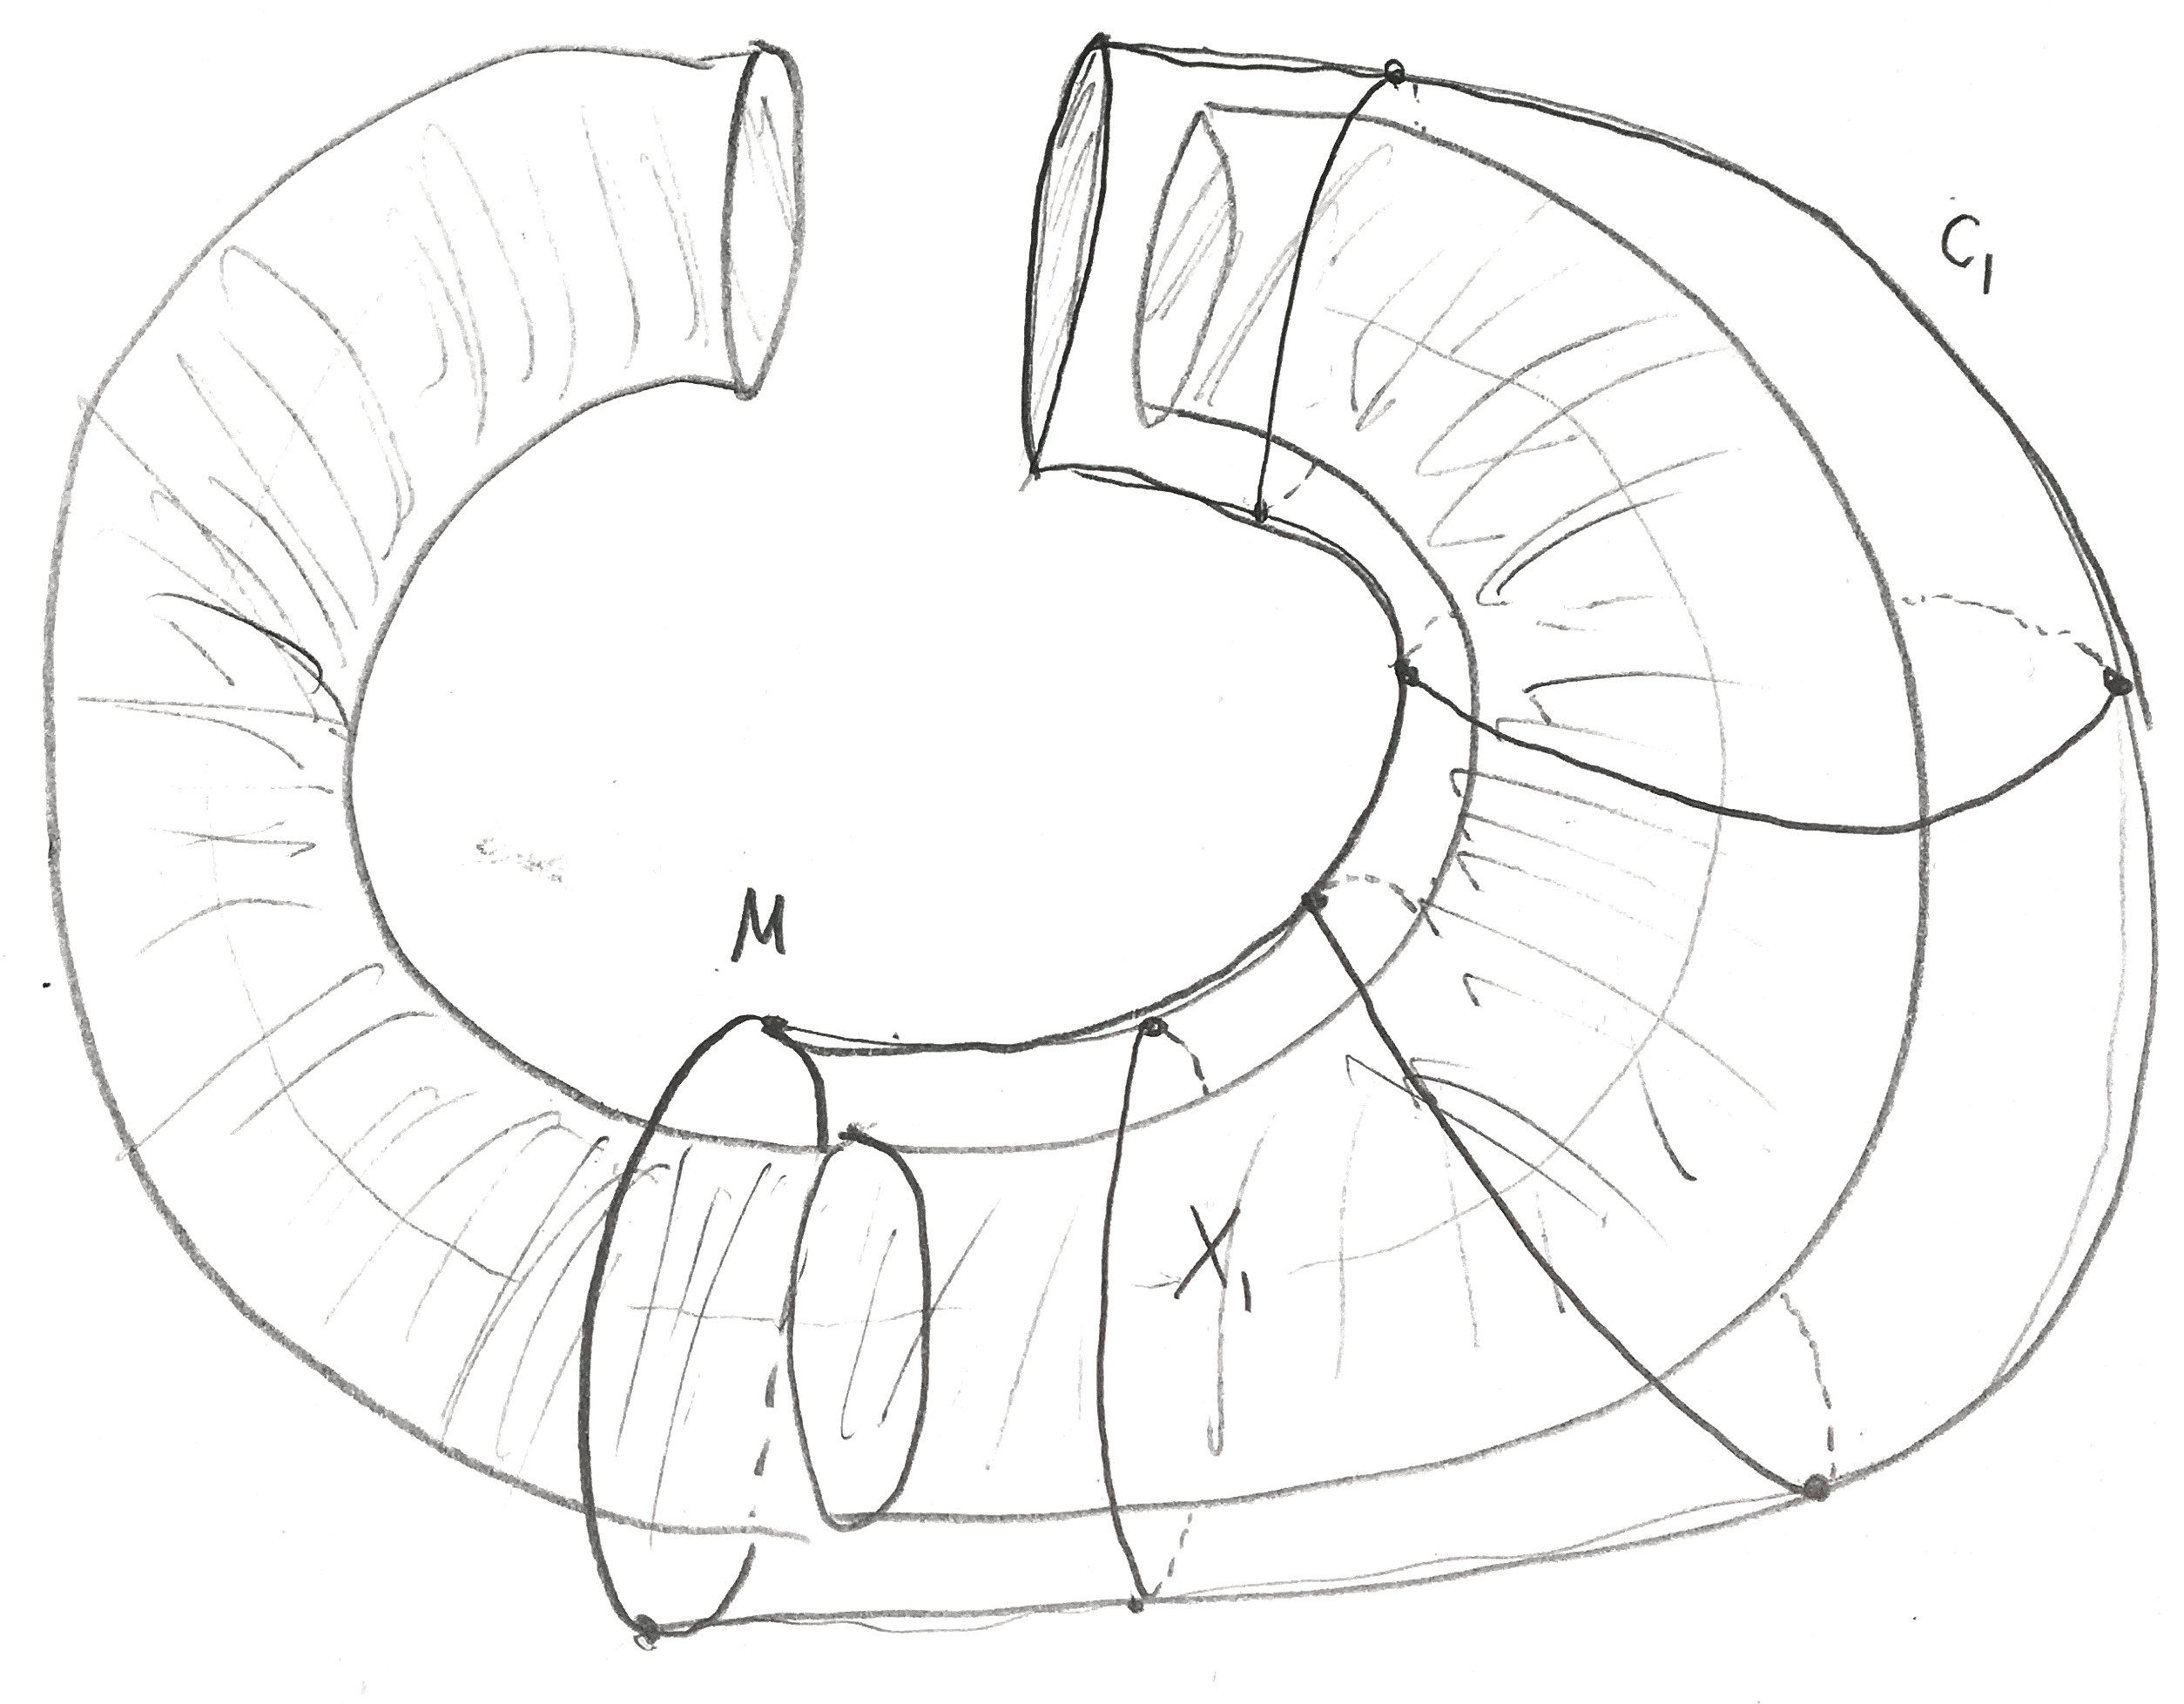
\includegraphics[width=0.5\textwidth]{s2.png}
  \end{center}
  In stage two we stretch $c_1$ so that $c_2$ wraps the two new horns on the right \emph{without} intersection the two new horns on the left as shown below.
    \begin{center}
  	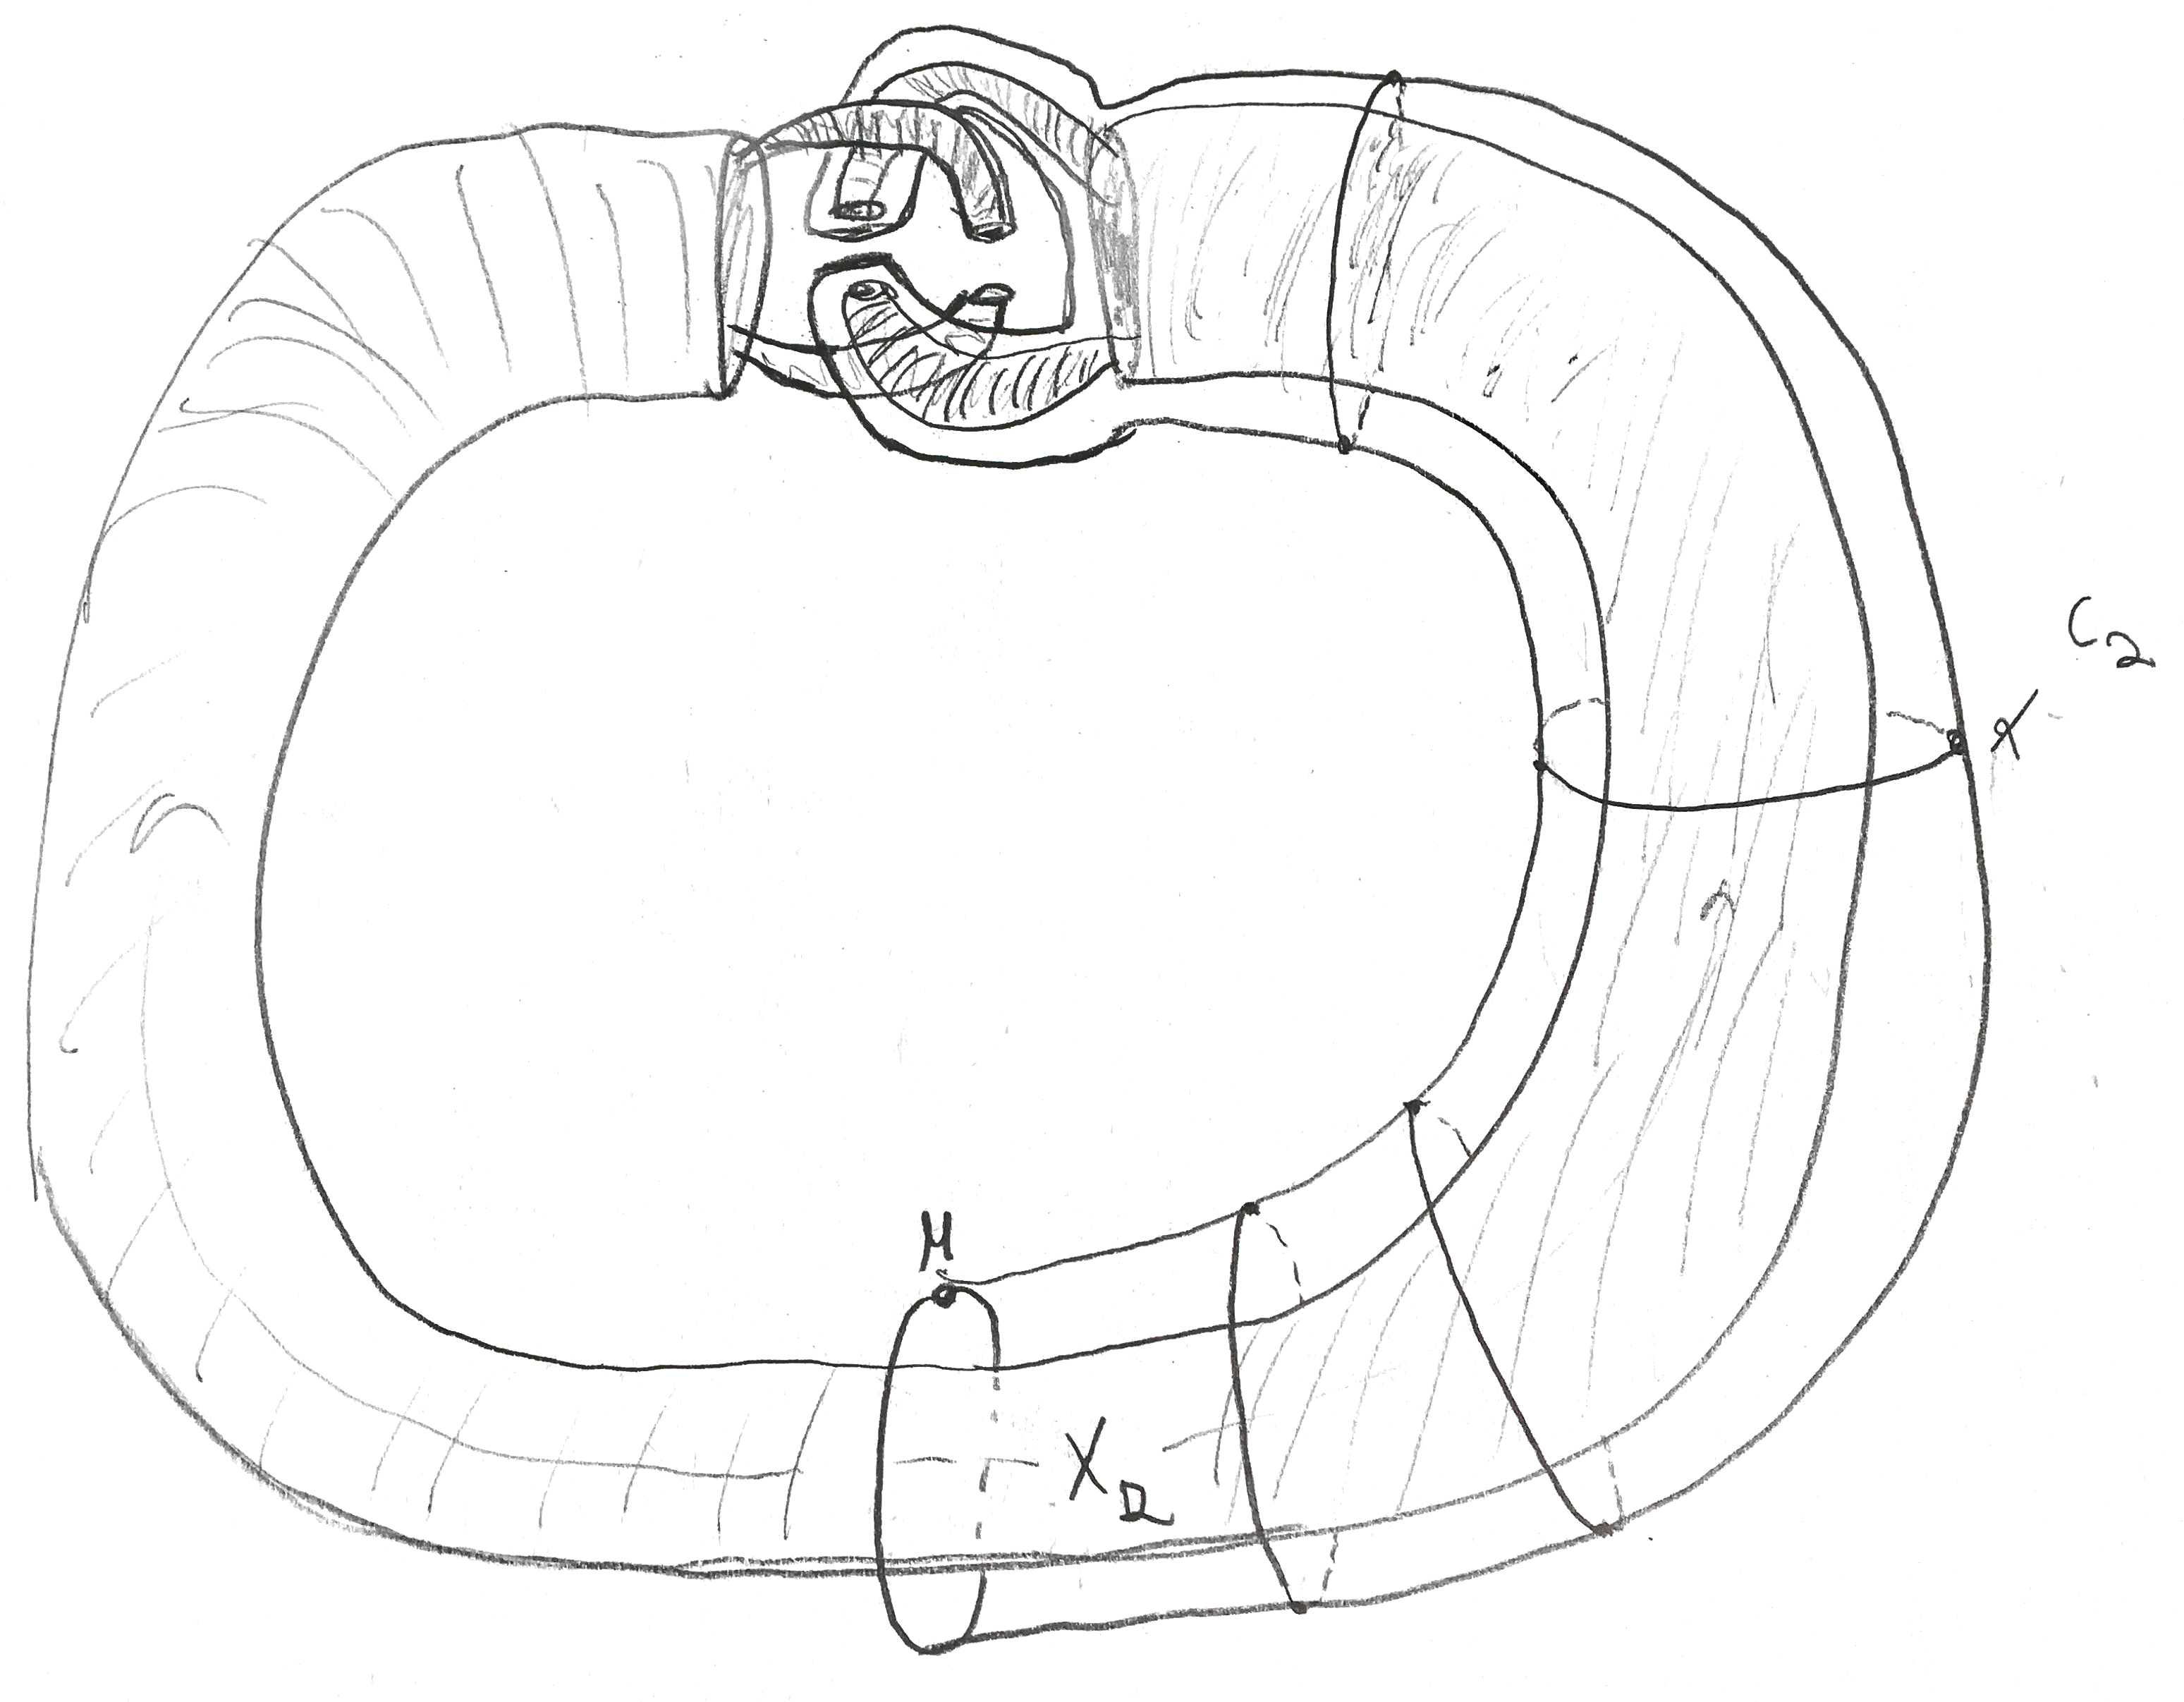
\includegraphics[width=0.5\textwidth]{s1.png}
  \end{center}
  At every stage $s_n$ we can perform this stretching to suround the two new horns as the compliment of the whole stage is open, and the horns on either side do not intersect. Each stage of this construction has a natural homeomorphism $h_n: c_n \to c_{n+1}$, where $h_n$ is the identity outside of a small neighborhood of $c_{n+1} - c_{n}$. Essentially $h_n$ just moves smaller and smaller ends of horns in $h_n$ to wrap the two new horns at the cooresponding neighborhood in $X_{n+1}$. Using the same argument as in the construction of horned ball $ \mathbb{R}^3 \setminus C $, the compositions of these homeomorphisms yield a uniformly convergent\footnote{Note that the $h_n$ only moves those $2^n$ small neighborhoods as aformentioned.} sequence of functions for which the limit $g: S^1 \setminus (D^1)^o \to C$ is injective. Using the compactnesss ofthe domain $g$ is then an embedding of its domain to its image in $C.$ We contend therefore $c:= g[S^1 \setminus (D^1)^o]$ is a compact oriented manifold.  Any orientable manifold with a boundary $\mu$ can be constructed by performing a connecting sum of tori or additional balls at each stage $c_n$ so it suffices to just consider our construction. 

  Since $\mu$ is the boundary of a compact oriented manifold, in particular an embedding of $S^1 \setminus (D^1)^o \cong \bar{D^1}$, then it $\mu \in Im(\partial_2)$ in the singular homology; thus $H_1(C) = Ker(\partial_1)/Im(\partial_2)$ implies that $\mu \sim 0$ is trivial as an element of the homology of $C$\footnote{At this point I realize that a discussion of other oriented manifolds, whose boundry is $\mu$, is not necisarry; we only need one to show that $\mu$ is a trivial element of the homology. }.


 \end{document}\end
